\documentclass[border=6pt]{standalone}
\usepackage{amsmath}
\usepackage{amssymb}
\usepackage{tikz}
\usetikzlibrary{arrows.meta,calc,decorations.pathreplacing,patterns,shapes.geometric,positioning,shadings,plotmarks}

\begin{document}
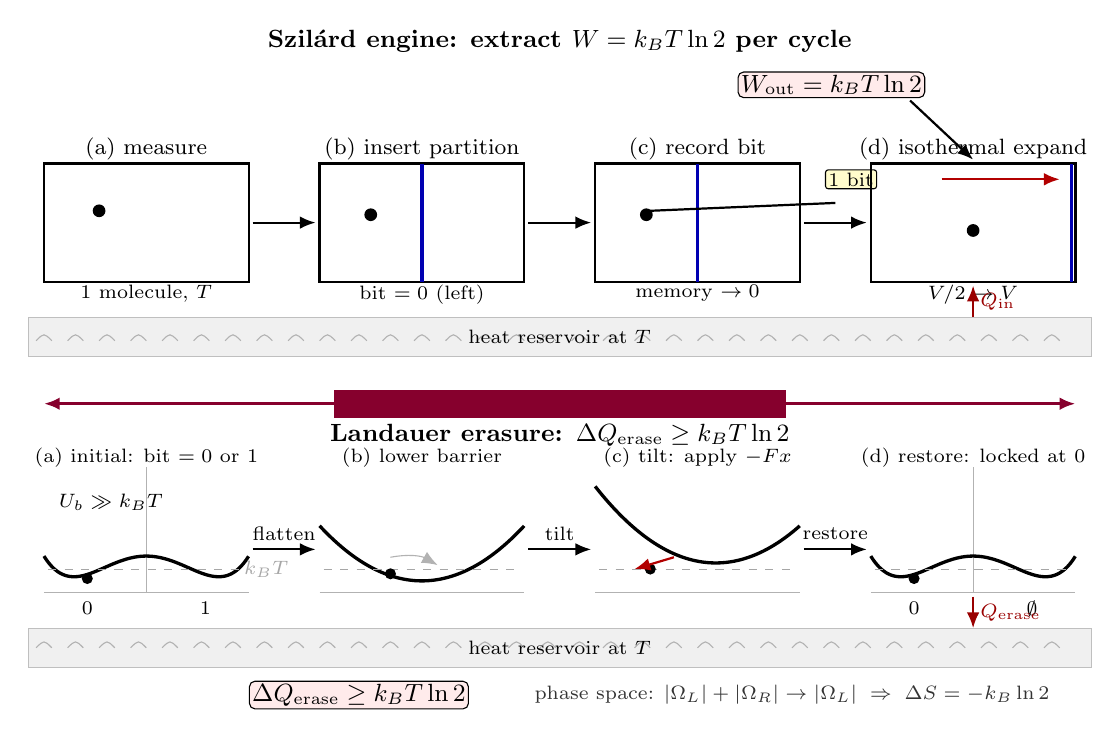
\begin{tikzpicture}[
  >={Latex[length=2mm,width=1.6mm]},
  font=\footnotesize,
  every node/.style={inner sep=1pt}
]

% =====================================================
% TOP ROW: Szilard engine 4-step cycle
% Panel widths cw=2.6, separation 0.9
% Panel x-origins: a=0, b=3.5, c=7.0, d=10.5; cell height 1.5; vertical center cy=3.3
% =====================================================
\node[font=\small\bfseries] at (6.55, 5.6) {Szil\'ard engine: extract $W = k_B T \ln 2$ per cycle};

% --- Step (a): single molecule, position random ---
\draw[thick] (0,2.55) rectangle (2.6,4.05);
\fill[black] (0.7, 3.45) circle (2.3pt);
\node[above] at (1.3, 4.05) {(a) measure};
\node[below, font=\scriptsize] at (1.3, 2.55) {1 molecule, $T$};

% --- Step (b): insert partition ---
\draw[thick] (3.5,2.55) rectangle (6.1,4.05);
\draw[very thick, blue!70!black] (4.8, 2.55) -- (4.8, 4.05);
\fill[black] (4.15, 3.4) circle (2.3pt);
\node[above] at (4.8, 4.05) {(b) insert partition};
\node[below, font=\scriptsize] at (4.8, 2.55) {bit $=0$ (left)};

% --- Step (c): demon sees, label 1 bit ---
\draw[thick] (7.0,2.55) rectangle (9.6,4.05);
\draw[very thick, blue!70!black] (8.3, 2.55) -- (8.3, 4.05);
\fill[black] (7.65, 3.4) circle (2.3pt);
% demon line of sight
\draw[thick] (10.05, 3.55) -- (7.7, 3.45);
\node[draw, fill=yellow!20, font=\scriptsize, rounded corners=1pt] at (10.25, 3.85) {1 bit};
\node[above] at (8.3, 4.05) {(c) record bit};
\node[below, font=\scriptsize] at (8.3, 2.55) {memory $\rightarrow 0$};

% --- Step (d): partition slides, isothermal expansion ---
\draw[thick] (10.5,2.55) rectangle (13.1,4.05);
\draw[very thick, blue!70!black] (13.05, 2.55) -- (13.05, 4.05);
\draw[->, thick, red!70!black] (11.4, 3.85) -- (12.9, 3.85);
\fill[black] (11.8, 3.2) circle (2.3pt);
\node[above] at (11.8, 4.05) {(d) isothermal expand};
\node[below, font=\scriptsize] at (11.8, 2.55) {$V/2 \to V$};

% Heat bath strip below top row (y center about 1.85)
\draw[fill=gray!12, draw=gray!50] (-0.2, 1.6) rectangle (13.3, 2.1);
\foreach \x in {0,0.4,...,13.0}{
  \draw[gray!60, thin] ($(-0.1+\x, 1.8)$) .. controls +(0.1,0.1) and +(-0.1,0.1) .. ($(0.1+\x, 1.8)$);
}
\node[font=\scriptsize] at (6.55, 1.85) {heat reservoir at $T$};

% Arrows between top steps
\draw[->, thick] (2.65, 3.3) -- (3.45, 3.3);
\draw[->, thick] (6.15, 3.3) -- (6.95, 3.3);
\draw[->, thick] (9.65, 3.3) -- (10.45, 3.3);

% Heat absorbed arrow (from bath to step d)
\draw[->, thick, red!60!black] (11.8, 2.1) -- (11.8, 2.5);
\node[right, font=\scriptsize, red!60!black] at (11.85, 2.3) {$Q_{\mathrm{in}}$};

% W = kT ln 2 label
\node[draw, fill=red!8, rounded corners=2pt, font=\small] at (10.0, 5.05) {$W_{\mathrm{out}} = k_B T \ln 2$};
\draw[->, thick] (11.0, 4.85) -- (11.8, 4.10);

% =====================================================
% Middle: bidirectional duality arrow at y = 1.05
% =====================================================
\draw[<->, very thick, purple!70!black] (0.0, 1.0) -- (13.1, 1.0);
\node[fill=white, font=\small\itshape, purple!70!black] at (6.55, 1.0) {two faces of information: $W_{\mathrm{out}} = Q_{\mathrm{erase}}$};

% =====================================================
% BOTTOM ROW: Double-well memory erasure
% Panel x-origins same as top: 0, 3.5, 7.0, 10.5; panel width 2.8 (so right edge 2.8); use 2.6 effective
% Baseline y = -1.4; panel height 1.6; top y = 0.2
% =====================================================
\node[font=\small\bfseries] at (6.55, 0.6) {Landauer erasure: $\Delta Q_{\mathrm{erase}} \ge k_B T \ln 2$};

% --- Panel A: symmetric double well ---
\draw[thin, gray!60] (0, -1.4) -- (2.6, -1.4);
\draw[thin, gray!60] (1.3, -1.4) -- (1.3, 0.2);
% double-well curve
\draw[very thick] plot[domain=0:1, samples=80, smooth]
  ({0 + \x*2.6}, {-1.25 + 1.05*( 16*(\x-0.5)^4 - 4*(\x-0.5)^2 + 0.30 )});
% dashed kT line
\draw[dashed, gray!70] (0.05, -1.10) -- (2.55, -1.10);
\node[right, font=\scriptsize, gray!70] at (2.5, -1.10) {$k_B T$};
% ball in left well
\fill[black] (0.55, -1.22) circle (2pt);
% labels 0 / 1
\node[font=\scriptsize] at (0.55, -1.6) {$0$};
\node[font=\scriptsize] at (2.05, -1.6) {$1$};
\node[above, font=\scriptsize] at (1.3, 0.15) {(a) initial: bit $=0$ or $1$};
\node[font=\scriptsize] at (0.85, -0.25) {$U_b \gg k_B T$};

% --- Panel B: barrier flattened, single broad well ---
\draw[thin, gray!60] (3.5, -1.4) -- (6.1, -1.4);
\draw[very thick] plot[domain=0:1, samples=80, smooth]
  ({3.5 + \x*2.6}, {-1.25 + 0.7*(2*(\x-0.5))^2});
\draw[dashed, gray!70] (3.55, -1.10) -- (6.05, -1.10);
\fill[black] (4.4, -1.16) circle (2pt);
% wandering arrow
\draw[->, thin, gray!60] (4.4, -0.95) to[bend left=20] (5.0, -1.05);
\node[above, font=\scriptsize] at (4.8, 0.15) {(b) lower barrier};

% --- Panel C: tilted potential, ball slides left ---
\draw[thin, gray!60] (7.0, -1.4) -- (9.6, -1.4);
\draw[very thick] plot[domain=0:1, samples=80, smooth]
  ({7.0 + \x*2.6}, {-1.25 + 0.7*(2*(\x-0.5))^2 + 0.5*(1-\x) });
\draw[dashed, gray!70] (7.05, -1.10) -- (9.55, -1.10);
\fill[black] (7.7, -1.10) circle (2pt);
\draw[->, thick, red!70!black] (8.0, -0.95) -- (7.5, -1.10);
\node[above, font=\scriptsize] at (8.3, 0.15) {(c) tilt: apply $-Fx$};

% --- Panel D: barrier restored, ball locked left ---
\draw[thin, gray!60] (10.5, -1.4) -- (13.1, -1.4);
\draw[thin, gray!60] (11.8, -1.4) -- (11.8, 0.2);
\draw[very thick] plot[domain=0:1, samples=80, smooth]
  ({10.5 + \x*2.6}, {-1.25 + 1.05*( 16*(\x-0.5)^4 - 4*(\x-0.5)^2 + 0.30 )});
\draw[dashed, gray!70] (10.55, -1.10) -- (13.05, -1.10);
\fill[black] (11.05, -1.22) circle (2pt);
\node[font=\scriptsize] at (11.05, -1.6) {$0$};
\node[font=\scriptsize] at (12.55, -1.6) {$\emptyset$};
\node[above, font=\scriptsize] at (11.8, 0.15) {(d) restore: locked at $0$};

% Arrows between bottom steps
\draw[->, thick] (2.65, -0.85) -- (3.45, -0.85);
\node[font=\scriptsize] at (3.05, -0.65) {flatten};
\draw[->, thick] (6.15, -0.85) -- (6.95, -0.85);
\node[font=\scriptsize] at (6.55, -0.65) {tilt};
\draw[->, thick] (9.65, -0.85) -- (10.45, -0.85);
\node[font=\scriptsize] at (10.05, -0.65) {restore};

% Heat bath below bottom row (y center about -2.1)
\draw[fill=gray!12, draw=gray!50] (-0.2, -2.35) rectangle (13.3, -1.85);
\foreach \x in {0,0.4,...,13.0}{
  \draw[gray!60, thin] ($(-0.1+\x, -2.10)$) .. controls +(0.1,0.1) and +(-0.1,0.1) .. ($(0.1+\x, -2.10)$);
}
\node[font=\scriptsize] at (6.55, -2.10) {heat reservoir at $T$};

% Heat dumped arrow from panel D to bath
\draw[->, thick, red!60!black] (11.8, -1.45) -- (11.8, -1.85);
\node[right, font=\scriptsize, red!60!black] at (11.85, -1.65) {$Q_{\mathrm{erase}}$};

% Landauer label box
\node[draw, fill=red!8, rounded corners=2pt, font=\small] at (4.0, -2.7) {$\Delta Q_{\mathrm{erase}} \ge k_B T \ln 2$};

% Phase-space note
\node[font=\scriptsize, gray!40!black] at (9.5, -2.7)
  {phase space: $|\Omega_L|+|\Omega_R| \to |\Omega_L|\;\Rightarrow\;\Delta S = -k_B \ln 2$};

\end{tikzpicture}
\end{document}
